\documentclass[tikz,border=2pt]{standalone}
\usepackage{amsmath}
\usepackage{amssymb}
\usetikzlibrary{arrows.meta}
\begin{document}
% Closed two-station cycle with n=3 jobs, E[S_1]=2 (mu_1=1/2), E[S_2]=1 (mu_2=1).
% State k = L_1 in {0,1,2,3}; k -> k+1 at rate mu_2 (k<3), k -> k-1 at rate mu_1 (k>0);
% level crossing gives p(k) proportional to 2^k, i.e. p = (1,2,4,8)/15.
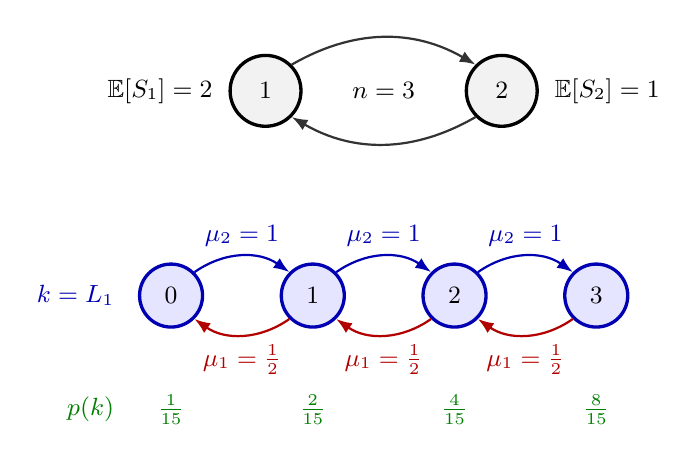
\begin{tikzpicture}[font=\small, >={Latex[length=2mm]},
  st/.style={circle, draw=black, very thick, fill=gray!10, minimum size=9mm},
  ks/.style={circle, draw=blue!70!black, very thick, fill=blue!10, minimum size=8mm}]
  % the network
  \node[st] (a) at (1.2,2.6) {$1$};
  \node[st] (b) at (4.2,2.6) {$2$};
  \draw[->, thick, gray!40!black] (a.north east) to[bend left=30] (b.north west);
  \draw[->, thick, gray!40!black] (b.south west) to[bend left=30] (a.south east);
  \node[anchor=east] at (0.65,2.6) {$\mathbb{E}[S_1]=2$};
  \node[anchor=west] at (4.75,2.6) {$\mathbb{E}[S_2]=1$};
  \node at (2.7,2.6) {$n=3$};
  % the state diagram of k = L_1
  \foreach \k in {0,1,2,3} { \node[ks] (k\k) at (1.8*\k,0) {$\k$}; }
  \foreach \k/\l in {0/1,1/2,2/3} {
    \draw[->, thick, blue!70!black] (k\k.north east) to[bend left=35] node[above] {$\mu_2=1$} (k\l.north west);
    \draw[->, thick, red!70!black] (k\l.south west) to[bend left=35] node[below] {$\mu_1=\tfrac{1}{2}$} (k\k.south east);
  }
  \node[anchor=east, blue!70!black] at (-0.6,0) {$k=L_1$};
  % stationary probabilities
  \node[anchor=east, green!50!black] at (-0.6,-1.45) {$p(k)$};
  \foreach \k/\v in {0/1,1/2,2/4,3/8} { \node[green!50!black] at (1.8*\k,-1.45) {$\tfrac{\v}{15}$}; }
\end{tikzpicture}
\end{document}
